\documentclass[12pt]{article}

\thispagestyle{empty}
\usepackage[scale=.95,landscape]{geometry}

\usepackage{amsmath}
\usepackage{fontspec}
\usepackage{unicode-math}
\setmainfont{TeX Gyre Bonum}
\setmathfont{TeX Gyre Bonum Math}

\usepackage{tcolorbox}
\usepackage{varwidth}

\usepackage{tikz}
\usetikzlibrary{
  matrix,
  matrix.skeleton,
  decorations.pathreplacing,
  calligraphy,
  positioning,
  arrows.meta,
  calc,
  fit,
  tikzmark
}

% Variance = 1/n \sum k^2 - (1/n \sum k)^2
% = 1/n ( n(n+1)(2n+1)/6 ) - (1/n n(n+1)/2)^2
% = (n+1)(2n+1)/6 - (n+1)^2/4
% = (n+1)( 2(2n+1) - 3(n+1) )/12
% = (n+1)(4n + 2 - 3n - 3) /12
% = (n+1)(n-1)/12

\usepackage{siunitx}
\usepackage{tikzpagenodes}

\usepackage{rational}

\DeclareMathOperator{\Var}{Var}

\ExplSyntaxOn

\rat_new:N \l__uniform_tmpa_rat

\cs_new_protected_nopar:Npn \uniform_row:nn #1#2
{
  \(\int_eval:n {#1}\) \&
  \(X \sim U(\int_eval:n {#1})\) \&
  \( \rat_display:n {1,#1+1,2} \) \&
  \( \rat_display:n {1,(#1+1)*(#1-1),12} \) \&
  \(\int_eval:n {#2}\) \&
  \(\frac{1}{\int_eval:n {#1}}\) \&
  \( \int_compare:nTF {#2 = 1} {0} { \rat_display:n {1,#2-1,#1} } \) \&
  \( \rat_display:n {1,#2,#1} \) \&
  \( \rat_display:n {1,#1 - #2+1,#1} \) \&
  \( \int_compare:nTF {#2 = #1} {0} { \rat_display:n {1,#1 - #2,#1} } \)
}
\cs_generate_variant:Nn \uniform_row:nn {VV}

\int_new:N \l__uniform_random_a_int
\int_new:N \l__uniform_random_b_int
\DeclareDocumentCommand \RandomUniformRow { m m }
{
  \int_set:Nn \l__uniform_random_a_int {\int_rand:n {#1/#2} * #2}
  \int_set:Nn \l__uniform_random_b_int {\int_rand:n { \l__uniform_random_a_int/#2} * #2}
  \uniform_row:VV \l__uniform_random_a_int \l__uniform_random_b_int
}
\DeclareDocumentCommand \UniformRow {m m}
{
  \uniform_row:nn {#1}{#2}
}

\DeclareDocumentCommand \RatDisplay {m}
{
  \rat_display:n {#1}
}

\ExplSyntaxOff

\tikzset{
  >=Latex,
  show cell/.style 2 args={
    row #1 column #2/.style={
      every node/.append style={text opacity=1}
    },
  },
  current row/.initial=1,
  step current row/.style={
    current row/.expanded={\the\numexpr\pgfkeysvalueof{/tikz/current row}+1\relax}
  },
  show cell on current row/.style={
    show cell={\pgfkeysvalueof{/tikz/current row}}{#1}
  },
  show cells/.style 2 args={
    current row=#1,
    show cell on current row/.list={#2}
  },
  show cells on next row/.style={
    step current row,
    show cell on current row/.list={#1}
  }
}

\begin{document}

\begin{center}
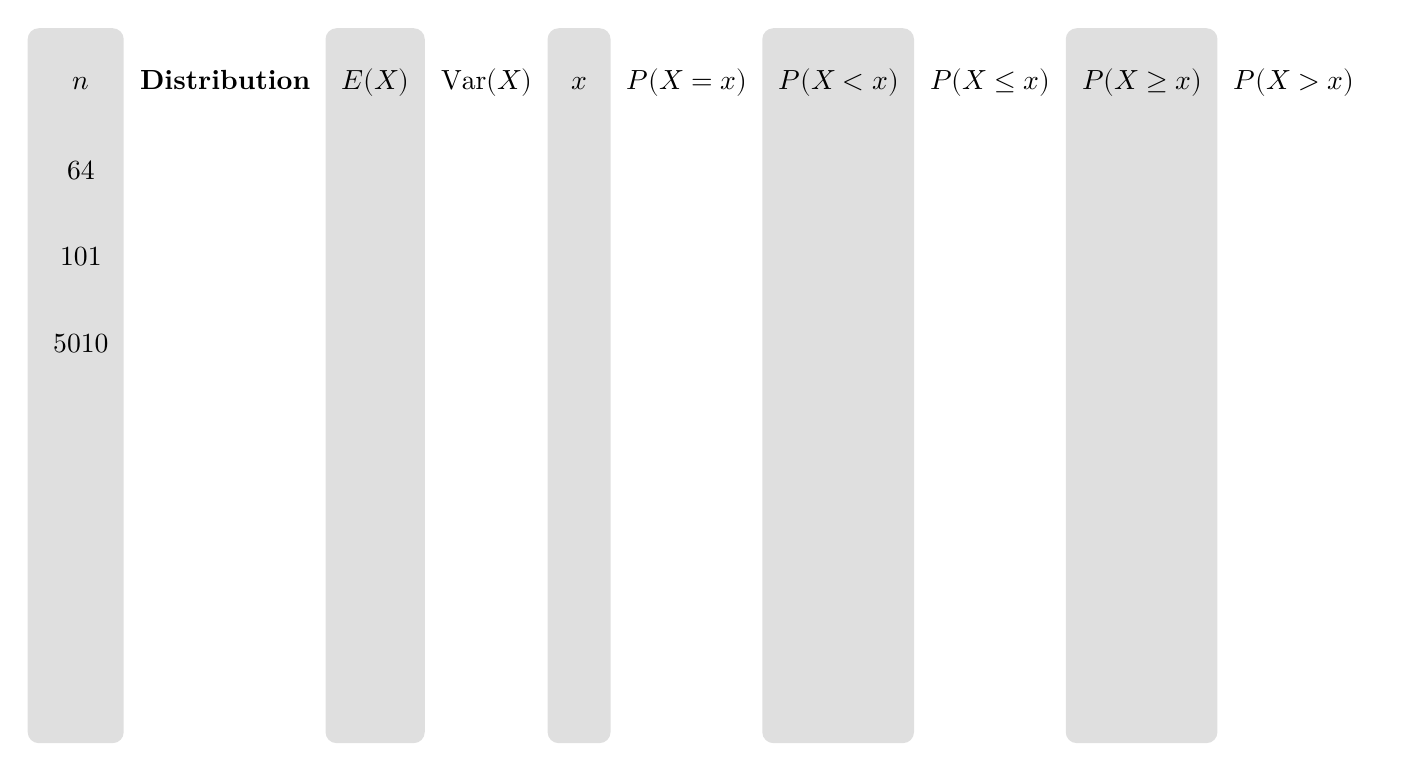
\begin{tikzpicture}
\matrix[
  matrix of nodes,
  ampersand replacement=\&,
  nodes={inner xsep=2mm, minimum width=.8cm,
    text opacity=0,
    minimum height=1.1cm},
  row 1/.style={every node/.append style={font=\bfseries,text opacity=1}},
  style odd tiling columns={fill=gray!25,rounded corners},
  %
  row 2/.style={every node/.append style={text opacity=1}},
  %
  current row=2,
  show cells on next row={1,5},
  show cells on next row={1,5},
  show cells on next row={3,5},
  show cells on next row={6,8},
  show cells on next row={8,9},
  show cells on next row={4,10},
]
(m)
{
  \(n\) \&
  Distribution \&
  \(E(X)\) \&
  \(\Var(X)\) \&
  \(x\) \&
  \(P(X = x)\) \&
  \(P(X < x)\) \&
  \(P(X \le x)\) \&
  \(P(X \ge x)\) \&
  \(P(X > x)\) \\
  %
  \UniformRow{6}{4} \\
  \RandomUniformRow{10}{1} \\
  \RandomUniformRow{50}{10} \\
  \RandomUniformRow{100}{5} \\
  \RandomUniformRow{100}{5} \\
  \RandomUniformRow{100}{1} \\
  \RandomUniformRow{100}{1} \\
};

\end{tikzpicture}
\end{center}



\end{document}
